\section{Funcões de Várias Variáveis}


Uma \dt{função real $f$ de $n$ variáveis} é uma relação que associa a cada $n$-upla $(x_1,\ldots,x_n)\in D\subset \R^n$ um único  número real $z=f(x_1,\ldots,x_n)$. O subconjunto $D$ de $\R^n$ é chamado \dt{domínio} da função $f$. Podemos denotar a função $f$ por
\[\begin{array}{ccl}
f:& D\subset\R^n & \longrightarrow \R\\
& (x_1,\ldots,x_n) & \longmapsto z=f(x_1,\ldots,x_n)
\end{array}\]


\begin{center}
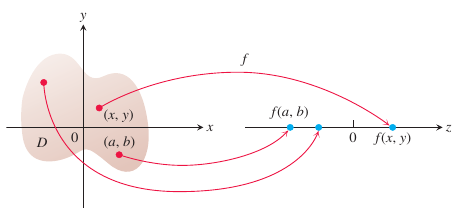
\includegraphics[scale=1]{figuras/func.png}
\end{center}


\begin{exeb}{}{}
 \begin{enumerate}
\item A função $V(r,h)=\pi r^2h$, $r,h>0$ é uma função de duas variáveis que  fornece o volume de um cilindro circular reto de raio da base $r$ e altura $h$.

 \item A função $z=f(x,y)=\frac{1}{x-y}$ é uma função de duas variáveis cujo domínio são todos os pontos $(x,y)\in \R^2$ tais que $x\neq y$.

 \item A função $\displaystyle f(x,y,z)=\frac{1}{(x^2+y^2+z^2)^{3/2}}$ é uma função de três variáveis cujo domínio são todos os pontos $(x,y,z)\in \R^3$ tais que $x^2+y^2+z^2\neq 0$, ou seja, $\R^3\setminus\{0\}$.

 \end{enumerate}
 \end{exeb}

\newpage
\marcador{subsection}{Gráfico de função}

O \dt{gráfico de uma função} $f:D\subset \R^2\to \R$, denotado por $G_f$, é o subconjunto do $\R^{3}$ formado por todos os pontos  da forma $(x,y,f(x,y))$, isto é,
\[G_f:=\{(x,y,z)\in \R^{3};\ z=f(x,y),\ (x,y)\in \R^2\}\]

\begin{center}
	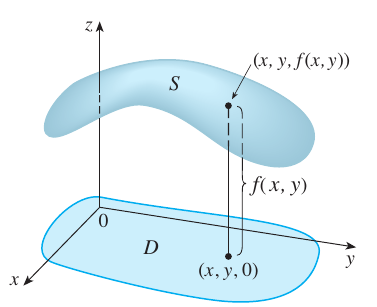
\includegraphics[scale=1]{figuras/grafico-f.png}
\end{center}

\begin{exeb}{}{}
\begin{enumerate}
\item Esboce a porção do gráfico da função  $f(x,y)=6-3x-2y$ que se encontra no primeiro octante.
\item Determine o domínio e esboce o gráfico da função \(g(x,y)=\sqrt{9-x^2-y^2}\).
\item Determine o domínio e o gráfico da função \(h(x,y)=4x^2+y^2\).
\end{enumerate}
\end{exeb}
\newpage

A seguir vemos uma série de gráficos de funções, gerados por um computador.
\begin{center}
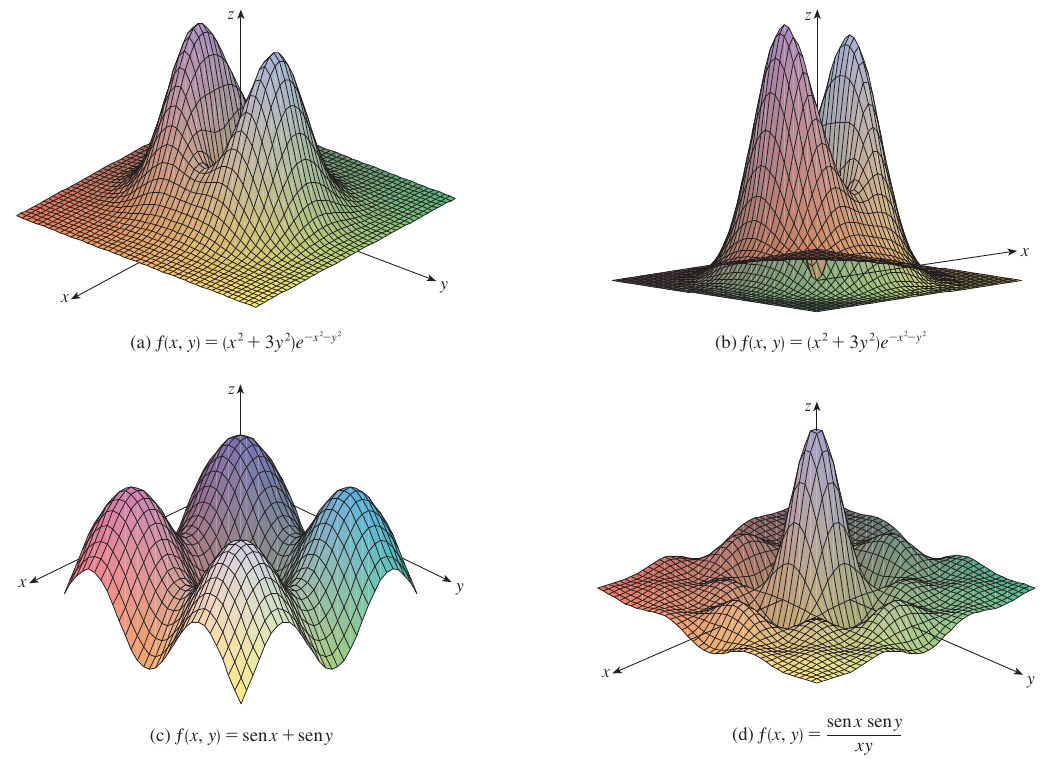
\includegraphics[scale=.7]{figuras/funcoes/graficos.png}
\end{center}



\newpage
\marcador{subsection}{Curvas de Nível}

Uma curva ao longo da qual uma função $z=f(x,y)$ tem valor constante é denominada \dt{curva de nível} da função $f$.

\begin{center}
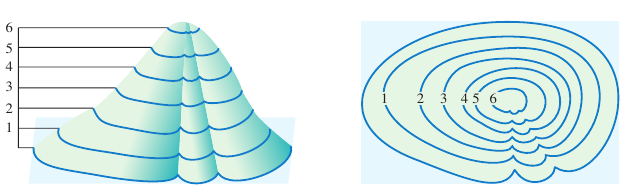
\includegraphics[scale=1]{figuras/nivel1.png}
\end{center}

 Quando a função $f$ representa a temperatura, as curvas de nível de $f$ são chamadas \dt{isotermas}. Se $f$ representa o potencial elétrico, as curvas de nível de $f$ são ditas \dt{curvas equipotenciais}. A equação da curva de nível ao longo da qual a função assume valor constante $k$ é
$$f(x,y)=k.$$
Se $S$ é a superfície do gráfico de uma função $f$, um conjunto de curvas de nível de uma função $f$ é dito \dt{um mapa de contorno da superfície $S$}.

\begin{center}
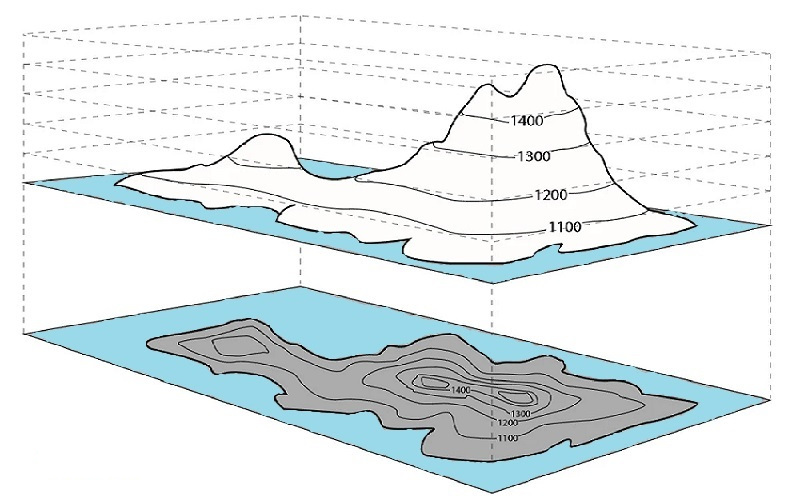
\includegraphics[scale=.8]{figuras/nivel3.jpg}
\end{center}
\newpage

\begin{exeb}{}{}
		A temperatura em cada ponto $(x,y)$ de uma placa de metal plana é dada, em graus, pela função $T(x,y)=4x^2+y^2$. Faça uma mapa de contorno das isotermas.
\end{exeb}

\begin{center}
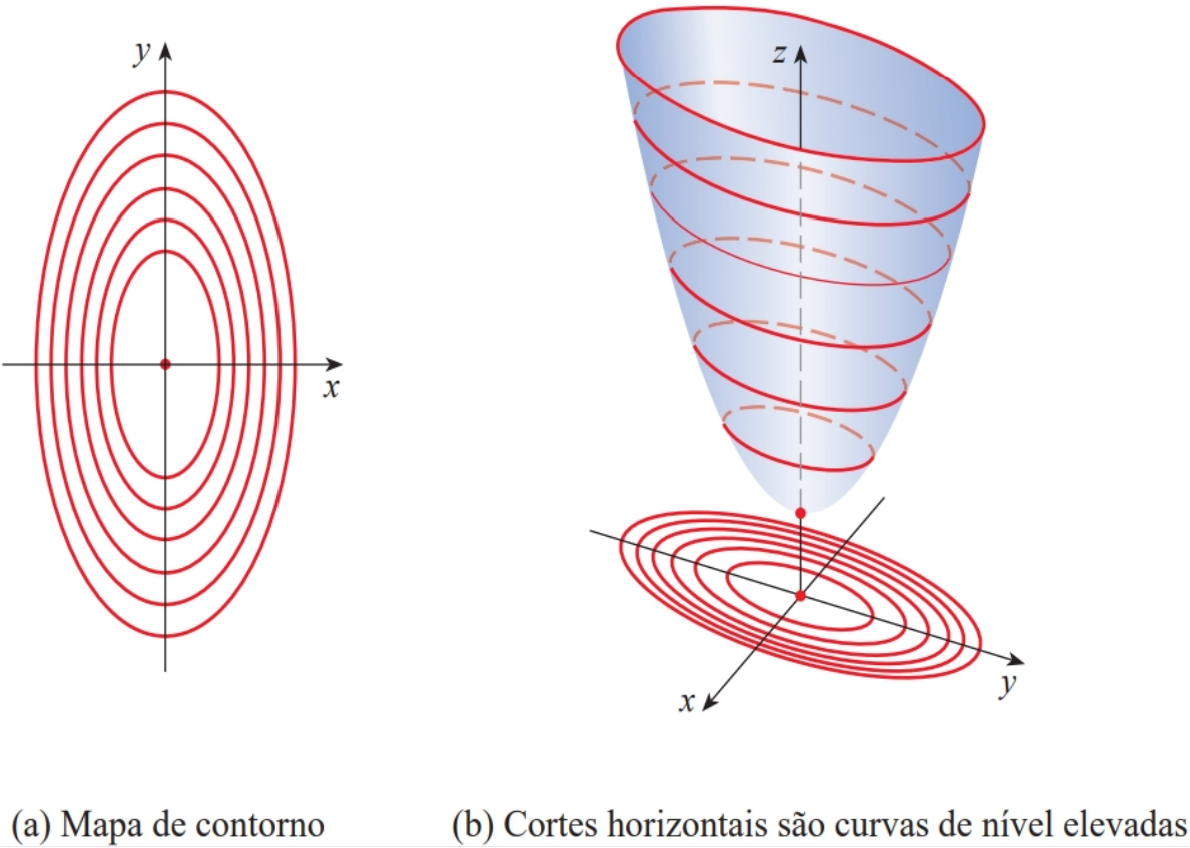
\includegraphics[scale=0.5]{figuras/funcoes/curva-nivel.png}
\end{center}
\newpage

\begin{center}

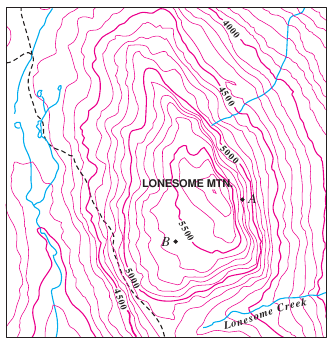
\includegraphics[scale=1]{figuras/nivel2.png}

Mapa topográfico de uma região montanhosa.

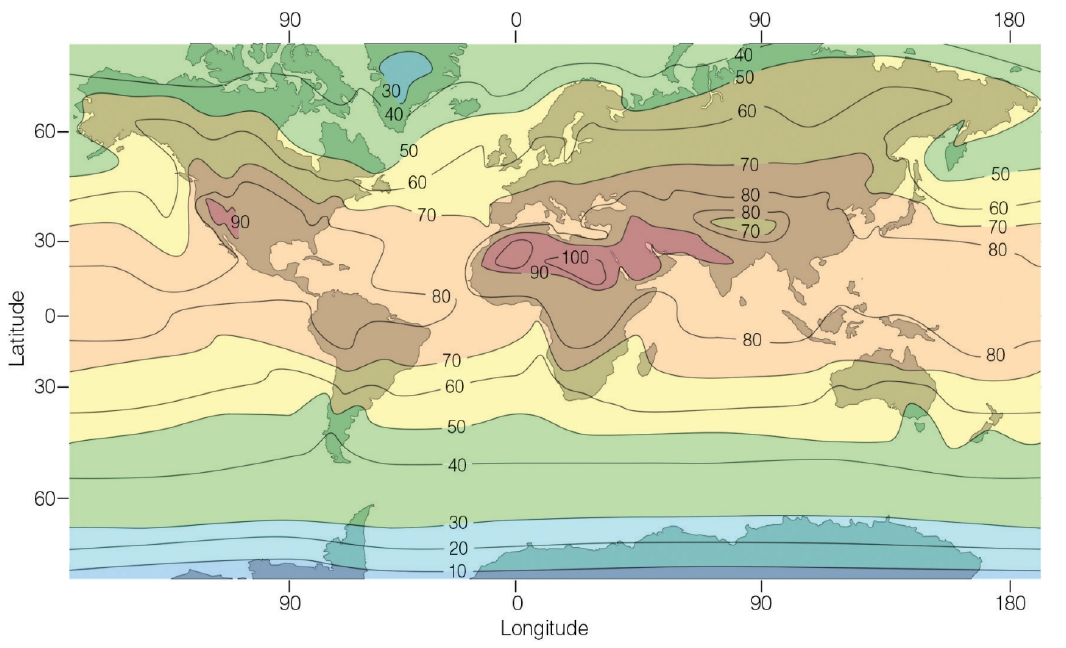
\includegraphics[scale=0.6]{figuras/nivel3.png}

Temperatura média do ar ao nível do mar no mês de julho em Fahrenheit

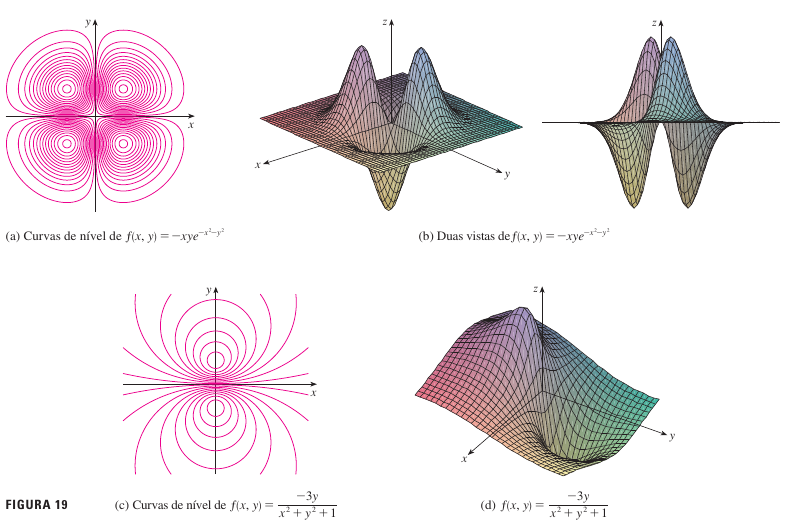
\includegraphics[scale=1]{figuras/nivel4.png}

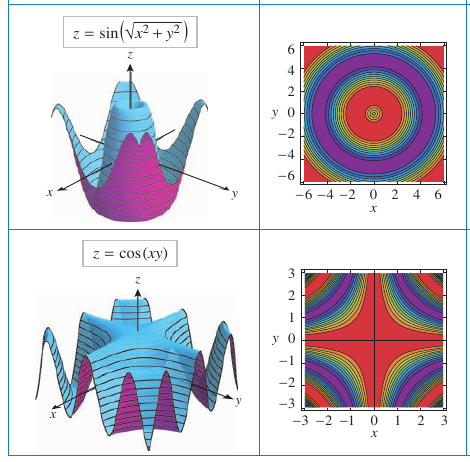
\includegraphics[scale=1]{figuras/nivel5.png}

Degradê de cores para indicar os níveis. Varia do roxo para o vermelho na ordem crescente.

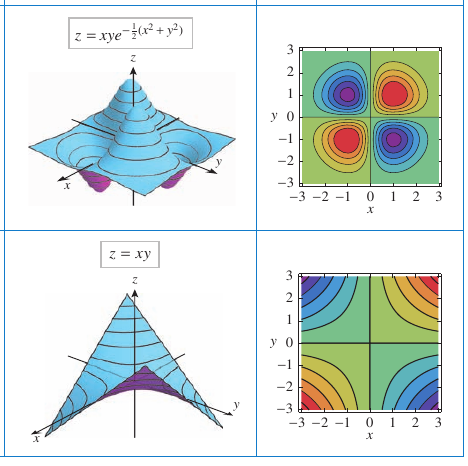
\includegraphics[scale=.9]{figuras/nivel6.png}
\end{center}

\newpage
\marcador{subsection}{Superfícies de Nível}

 No caso de funções de três variáveis, um conjunto no qual uma função $f(x,y,z)$ tem valor constante é dita \dt{uma superfície de nível} da função $f$.

\begin{exeb}{}{}
 Descreva as superfícies de nível da função $f(x,y,z)=x^2+y^2+z^2$.
\end{exeb}

\begin{center}
	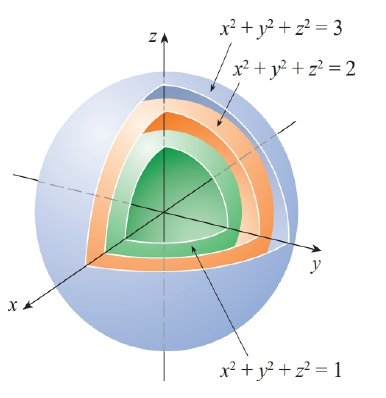
\includegraphics[scale=1]{figuras/nivel-superfice.png}
\end{center}

\begin{casab}{}{}
\begin{enumerate}
\item Esboce a região de domínio da função
\[f(x,y)=x\log(y^2-x)\]

\item Faça um mapa de contorno da função $f(x,y)=4-x^2-y$ para os níveis $5,4,3,2,1,0,-1$ e faça um esboço do gráfico.

\item Descreva as superfícies de nível da função $f(x,y,z)=z-x^2-y^2$.
\end{enumerate}
\end{casab}

